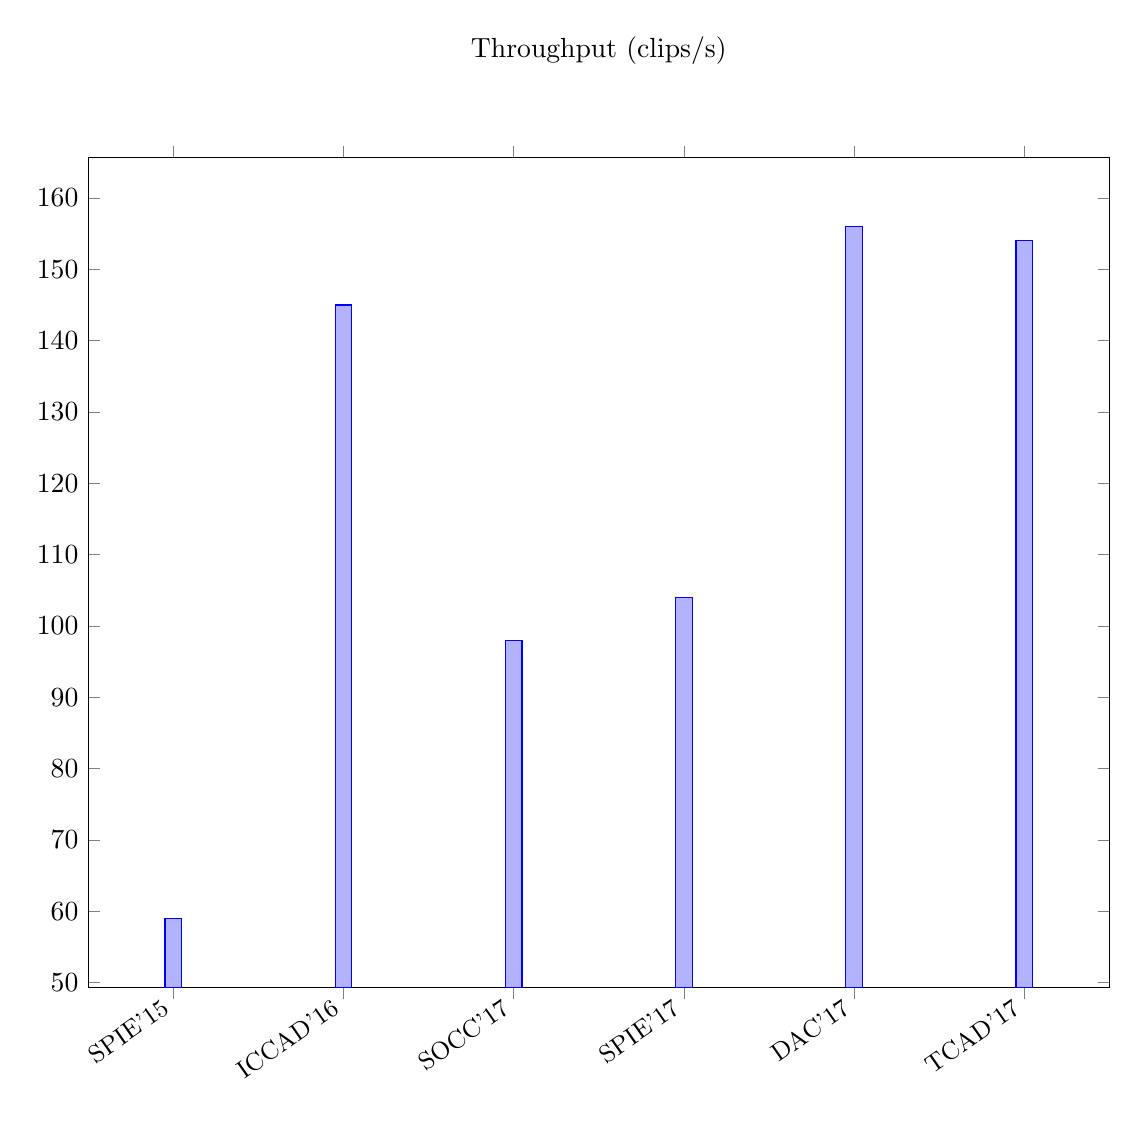
\begin{tikzpicture}
\pgfplotsset{
	width =1.2\textwidth,
	height=1\textwidth,
	every axis plot/.append style = {font = \tiny}
}
\begin{axis}[
ybar=2.5pt,
%enlargelimits=0.15,
bar width=6pt,
legend style={at={(0.5,-0.15)},
	anchor=north,legend columns=-1},
area legend,
ylabel={Throughput (clips/s)},
y label style={at={(axis description cs:0.5,1.1)},rotate=270,anchor=south},
symbolic x coords={SPIE'15,ICCAD'16,SOCC'17,SPIE'17,DAC'17,TCAD'17},
xtick=data,
x tick label style={rotate=35,anchor=east,font=\small},
%nodes near coords,
%nodes near coords align={vertical},
]
\addplot  coordinates {(SPIE'15,59) (ICCAD'16,145) (SOCC'17,98) (SPIE'17,104)(DAC'17,156)(TCAD'17,154)};

\end{axis}
\end{tikzpicture}
